\chapter{The Schwinger model in a lattice}

\section{Motivation and Introduction}
 
 Lattice models in physics are versions of continuum field theories which are discretized to a lattice with the objective of making them useful for computer simulations. The motivation of this discretization procedure is that most quantum field theories are not exactly solvable and thus computer simulations can yield a great physical insight into the continuum theory. The aim is to take increasing system sizes while reducing the lattice spacing hoping that for a sufficiently fine discretization the continuum behavior of the model can be recovered. Moreover, numerical simulations can give access to non-trivial field configurations and vacuum states which are non-perturbative. The lattice version of gauge theory is particularly useful since gauge invariance is kept manifest at the Hamiltonian level \cite{Kogut1975}. The Schwinger model being a simple gauge theory is appealing to the methods of lattice gauge theory, and thus the exploration of its lattice version will be very useful to study the dynamics of the system.\\

In this chapter, we will study the discrete version the Schwinger using Kogut-Susskind fermions \cite{Kogut1975,Susskind1977}. Using the Hamiltonian form of the theory (cf. equation \eqref{eq:SchHAmil}) we will construct lattice Hamiltonian. Furthermore, we will show the equivalence of this Hamiltonian to a spin chain model, and how in the case of the free Schwinger model the Hamiltonian coincides with the XX-model.\\

Moreover, we will discuss how gauge invariance fixes the form of the Hamiltonian describing the dynamics of the gauge field which turns out to be a quantum rotor. We show how the inclusion of the background field $\mathcal{E}_0$ follows straightforwardly from the continuum Hamiltonian and that the lattice model inherits the same critical behavior induced by the dynamics of particle anti-particle pair production present in the continuum model.\\

Finally, we show how Gauss's law fixes the subspace of physical states of the theory. This restriction imposed by gauge invariance permits the elimination of the gauge field from the Hamiltonian altogether. However, this introduces an effective mass term and a Coulomb interaction term to the lattice Hamiltonian. This formulation absent pf the gauge field variables will prove extremely useful in the next chapter were the computer simulations of the lattice system will be discussed.

\section{Lattice formulation}\label{sec:latticeFormulation}

The Schwinger model can be discretized on an $N$ point lattice with lattice spacing $a$. We can work on either open, periodic or antiperiodic boundary conditions as seen in figures \ref{fig:latticeCond}

 \begin{figure}[htb]
     \centering
     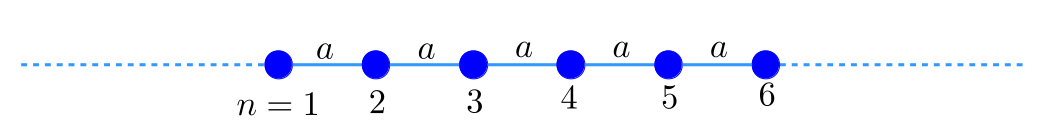
\includegraphics[scale=0.35]{figures/latice1.png}
     \centering
     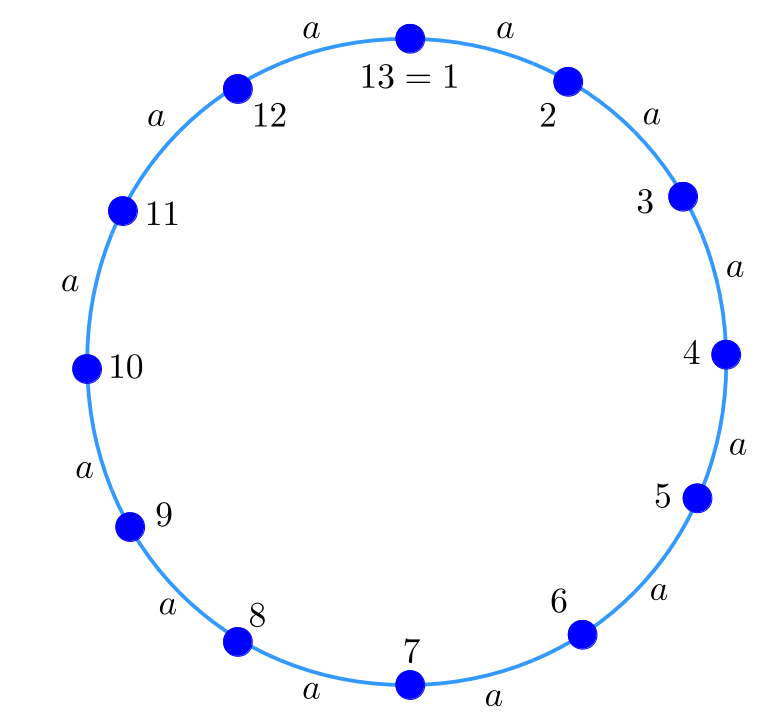
\includegraphics[scale=0.3]{figures/latice2.png}
    \caption{Lattice with open and periodic boundary condition.}
     \label{fig:latticeCond}
 \end{figure}
 

Using the gamma matrices representation \eqref{eq:gammarep2} the massless Dirac equation can be rewritten as

\begin{equation}
    \partial_t \psi =   \mqty(\admat[0]{1,1})\partial_x \psi.\label{eq:diraceq11}
\end{equation}

We can replace the spatial derivative  in \eqref{eq:diraceq11} by a discrete difference

\begin{equation}
     \partial_t \psi = \mqty(\admat[0]{1,1})\frac{1}{2a}\qty[\psi(n+1) - \psi(n-1)],\label{eq:discreteDirac}
\end{equation}

and then we can reduce the number of degrees of freedom in each site by introducing one-component fermions $\phi$ on each lattice site. We demand that $\phi$ obeys equation \eqref{eq:discreteDirac}. By using the Heisenberg equations of motion we find that $\phi$ must have the following Hamiltonian

\begin{equation}
H = \frac{-i}{2a} \sum_n \qty[\phi^\dagger_n \phi_{n+1} - \phi^\dagger_{n+1}\phi_n].
\end{equation}

Moreover, we can introduce Kogut-Susskind fermions \cite{Banks} on a staggered lattice by defining even and odd sub-lattices which have independent fermion fields related to $\phi$ by

\begin{align}
&\psi_- = \frac{1}{\sqrt a} \phi_n,\quad n\text{ even}\nonumber\\
&\psi_+= \frac{1}{\sqrt a} \phi_n,\quad n\text{ odd},
\end{align}

obeying 

\begin{equation}
    \partial_t \psi_\pm = \frac{1}{2a}\qty[\psi_\pm(n+1) - \psi_\pm(n-1)].
\end{equation}

Since the lattice is a staggered one, translation symmetry is represented by a shift of even lattice sites namely:

\begin{equation}
\psi_\pm(n)\to\psi_\pm(n+m),\quad\quad m\,\text{mod}2 =0.
\end{equation}
Within this formulation, fermion bilinears can be expressed in the lattice yielding

\begin{align}
	\psi^\dagger\psi &=\psi_-^\dagger(n)\psi_-(n) + \psi_+^\dagger(n)\psi_+(n) = \phi_n^\dagger\phi_n\nonumber\\
	\bar\psi\psi &= \psi_-^\dagger(n)\psi_-(n) - \psi_+^\dagger(n)\psi_+ (n)= (-1)^n\phi_n^\dagger\phi_n.\label{eq:latB}
\end{align}

Equation \eqref{eq:latB}, in particular, implies that a mass term in the Dirac equation $m\bar\psi\psi$ has the following lattice form

\begin{equation}
    m\sum_n (-1)^n\phi_n^\dagger\phi_n.
\end{equation}

\subsection{Spin Hamiltonians}

There exists a close connection between one-dimensional fermion chains and spin chains given by the Jordan-Wigner transformation. Let us think of a $1/2$-spin chain with Pauli spin operators $\sigma^\pm_n$ and $\sigma^z_n$, the Jordan-Wigner transformation  

\begin{align}
	\phi_n &= \qty[\prod_{l<n}i\sigma^z_l]\sigma^+_n\nonumber\\
	\phi_n^\dagger &= \qty[\prod_{l<n}-i\sigma^z_l]\sigma^-_n\label{eq:JWtrans}
\end{align}

relates the fermion operators with the spin operators. Hence, the fermion Hamiltonian is equivalent to the following spin Hamiltonian

\begin{equation}
H = J\sum_n \qty[\sigma^+_n\sigma^-_{n+1} + \sigma^+_{n+1}\sigma^-_n] = \frac{J}{2}\sum_n\qty[\sigma^x_n \sigma^x_{n+1} + \sigma^y_n \sigma^y_{n+1}],\label{eq:XXhamil}
\end{equation}

with $J=1/2a$. Hamiltonian \eqref{eq:XXhamil} is a special case of the XX-model Hamiltonian (with $\gamma=0$ and $g=0$) and whose solution we worked out in detail in chapter 2 (cf. section \ref{sec:XYmodel}). Hamiltonian \eqref{eq:XXhamil} is the lattice equivalent of the \emph{free massless} Schwinger model.\\

In terms of spin matrices, Dirac bilinears are expressed as 

\begin{align}
    \psi^\dagger\psi &= \frac{1}{2}\sigma^z_n,\nonumber\\
    \bar\psi\psi &= \frac{(-1)^n}{2}\qty(1+\sigma^z_n),\nonumber\\
    \psi^\dagger\gf\psi &= -i\qty(\sigma^+_n \sigma^-_{n+1} - \sigma^+_{n+1}\sigma^-_n),\nonumber\\
    i\bar{\psi}\gf\psi &= \qty(\sigma^+_{n+1} \sigma^-_{n} + \sigma^+_{n}\sigma^-_{n+1}),\label{eq:lattBiliSpin}
\end{align}

which implies that both charge densities are written as

\begin{align}
    J^0 &= \frac{1}{2}\comm{\psi^\dagger}{\psi} = \frac{1}{2}\sigma^z,\nonumber\\
    J_5^0 &= \psi^\dagger\gf\psi = -i\qty[\sigma^+_n\sigma^-_{n+1} + \sigma^+_{n+1}\sigma^-_{n}].
\end{align}

A straightforward modification of \eqref{eq:XXhamil} in virtue of \eqref{eq:lattBiliSpin} allows us to introduce the mass term, which in spin language is a staggered transverse field

\begin{equation}
H = J\sum_n\qty[\sigma^+_n\sigma^-_{n+1} + \sigma^+_{n+1}\sigma^-_n] + \frac{m}{2}\sum_n (-1)^n\sigma^z_n\label{eq:XXHamilMass}.
\end{equation}

This is the XY Hamiltonian with $\gamma=0$ and a staggered transverse field with $g=m/2$. Hamiltonian \eqref{eq:XXHamilMass} is the lattice equivalent of the \emph{massive free} Schwinger model. Thus far, we have just introduced the fermion part of \eqref{eq:SchHAmil}. This begs the question: how can we introduce the electromagnetic field in a gauge invariant manner?\\

To do so we use as inspiration the gauge invariant point-splitting method \eqref{eq:pointSplitting}. In gauge invariant point splitting in order to preserve the gauge invariance, one must multiply by a phase factor that exactly cancels the transformation term picked up by the spinors. This phase factor is of the form

\begin{equation*}
    \exp\qty[i q_e\int_x^{x+\epsilon}\dd{x}A_1].
\end{equation*}

Hence, following this prescription as a guide on how to proceed in the lattice we can on each link between lattice sites define the following operator

\begin{equation}
    U(n;n+1)  = e^{i\alpha_n}
\end{equation}

with $\alpha_n =i a q_e A_1(n)$. This will be the parallel transporter operator associated to the $U(1)$ gauge field. Recall, we are working in the gauge $A_0=0$, which implies that the electric field $E = -\dot{A_1}$ is the canonical conjugate variable of $A_1$. In the lattice formulation, this is equivalent to

\begin{equation}
    \comm{A_n}{E_m} = i q_e\delta_{n,m}\label{eq:commE1},
\end{equation}
 
and from relation \eqref{eq:commE1} we can define the following operator

\begin{equation}
L_n = \frac{E_n}{q_e}.
\end{equation}

It follows from \eqref{eq:commE1} that the  physical range of $\alpha_n$ is (cf. section \ref{sec:FermionSpectrum})

\begin{equation}
A_1 \in \qty[0,\frac{2\pi}{q_ea}]\quad \Rightarrow \quad \alpha_n \in [0,2\pi].
\end{equation}

Also, it follows that $L_n$ is an angular momentum operator which is quantized in integer values

\begin{equation}
L\ket{n}=l\ket{l};\quad l=0,\pm1,\pm2,\ldots.\label{eq:lQuant}
\end{equation}

Hence the electric field in the lattice version is represented by a \emph{quantum rotor} in each link in between the fermions.\\

To render the Hamiltonian \eqref{eq:XXHamilMass} gauge invariant, link operators $U$ are introduced in the same spirit of gauge invariant point-splitting

\begin{equation}
J\sum_n\qty[\sigma^+_n\sigma^-_{n+1} + \sigma^+_{n+1}\sigma^-_n] \to J\sum_n\qty[\sigma^+_n e^{i\alpha_n}  \sigma^-_{n+1} + \sigma^+_{n+1} e^{-i\alpha_n}\sigma^-_n],
\end{equation}

namely the Hamiltonian reads

\begin{equation}
H = J\sum_n\qty[\sigma^+_n e^{i\alpha_n}  \sigma^-_{n+1} + \sigma^+_{n+1} e^{-i\alpha_n}\sigma^-_n] + \frac{m}{2}\sum_n (-1)^n\sigma^z_n.
\end{equation}

Thus far, we have not introduced the dynamic Hamiltonian of the electric field. We introduce this term for the electromagnetic field to the lattice formulation following Hamiltonian \eqref{eq:SchHAmil}

\begin{equation}
H = J\sum_n\qty[\sigma^+_n e^{i\alpha_n}  \sigma^-_{n+1} + \sigma^+_{n+1} e^{-i\alpha_n}\sigma^-_n] + \frac{m}{2}\sum_n (-1)^n\sigma^z_n + \xi \sum_n L_n^2,\label{eq:fullHamiltonian}
\end{equation}

with $\xi = q_e^2 a/2$. This is the lattice equivalent of the \emph{fully interacting massive} Schwinger model.\\

\subsection{Electric field operators and Hilbert space}\label{ssec:operators}

 Let us note that both $\alpha_n$ and $A_1$ only appear in the Hamiltonian trough $e^{\pm\alpha_n}$. However, we need to determine how such operators act on the eigenstates of operator $L_n$. From the commutator \eqref{eq:commE1} we have that
 
 \begin{align}
 	\alpha_n L_n\ket{l} - L_n\alpha_n\ket{l} &= i\ket{l} \nonumber\\
 	l\alpha_n\ket{l} - L_n\alpha_n\ket{l} &= i\ket{l}\label{eq:ltheta}.
 \end{align}
 
 By acting upon \eqref{eq:ltheta} with $\alpha_n$ and using repeatedly \eqref{eq:commE1} we arrive to a relation of the form
 
 \begin{equation*}
 	l(\alpha_n)^k\ket{l} - L_n(\alpha_n)^k\ket{l} = i k (\alpha_n)^{k-1}\ket{l}.
 \end{equation*}
 
 If we multiply by $(\pm i)^k/k!$ and sum over all possible values of k we have that
 
 \begin{equation}
 l\sum_{k=1}^\infty\frac{(\pm i)^k}{k!} (\alpha_n)^k \ket{l} - L_n \sum_{k=1}^\infty\frac{(\pm i)^k}{k!} (\alpha_n)^k \ket{l}  = \sum_{k=1}^\infty\frac{(\pm i)^k}{k!} i k (\alpha_n)^{k-1}\ket{l},
 \end{equation}
 
 summing both the first and second sums form $k=0$ and making the change $k$ to $k+1$ in the right-hand side sum we obtain that
 
 \begin{equation}
 l\sum_{k=0}^\infty\frac{(\pm i)^k}{k!} (\alpha_n)^k \ket{l} - L_n \sum_{k=0}^\infty\frac{(\pm i)^k}{k!} (\alpha_n)^k \ket{l}  = \mp \sum_{k=0}^\infty\frac{(\pm i)^k}{k!} i k (\alpha_n)^{k}\ket{l},
 \end{equation}
 
 finally, using the definition of the exponential of an operator this is equivalent to
 
 \begin{equation}
 (l\pm1)e^{\pm i\alpha_n}\ket{l} = L_n e^{\pm i\alpha_n}\ket{l}.
 \end{equation}
 
 Therefore, we note that 
 
 \begin{equation}
 e^{\pm i\alpha_n}\ket{l} = C \ket{l+1}.
 \end{equation}
 
 If we further assume that states $\ket{l}$ form a complete orthonormal basis, then we can choose $C=1$. Hence, we have shown that the operators $e^{\pm i\alpha_n}$ are the \emph{raising (lowering) operators} of the eigenstates of $L_n$ \cite{Banks}.

These results suggest that the relevant Hilbert space of the lattice model is a tensor product of the spin space and the $L$-space of the quantum rotor that represents the electromagnetic field, viz

\begin{equation}
    \mathscr{H} =\bigotimes_{i=1}^N\ket{s_i}\otimes \ket{l}.
\end{equation}

Here $s_i=\{\uparrow,\downarrow\}$ label the $\pm1$ eigenstates of $\sigma^z$ and $l\in\mathbb{Z}$. As a consequence of the staggered nature of the lattice, an even site in spin state $\ket{1}$ has a fermion (an electron) while an odd site in spin state $\ket{0}$ corresponds to an anti-fermion (a positron).

\subsection{The background field in the lattice}

As it was discussed in section \ref{ssec:BackgroundField} very interesting physics arises when we consider the presence of a background electric field as a consequence of the dynamics of pair production in one spatial dimension. The lattice version of the Schwinger model as described by the Hamiltonian \eqref{eq:fullHamiltonian} inherits this interesting physical behavior as well. The modification is simple,  as it amounts to adding a single term in the Hamiltonian to account for the electrostatic energy of the background electric field, hence the kinetic term for the electromagnetic field is modified to

\begin{equation}
\xi\sum_n L_n^2 \to  \xi\sum_n (L_n + \mathcal{E}_0)^2.
\end{equation}

Thus, by virtue of this modification the physics of the lattice model in the presence of the background field corresponds exactly with the continuum model. If $\mathcal{E}_0 >1/2$, pair production will begin and opposite charges separate the spatial edges lowering the electrostatic vacuum energy and bringing $\mathcal{E}_0$ below $1/2$. Therefore, at $\mathcal{E}_0=1/2$ a phase transition occurs between two degenerate ground states above the critical mass \cite{Byrnes2002}

\begin{equation}
    m_c = \frac{m}{q_e} = 0.3335(2).
\end{equation}

In this context of spontaneous symmetry breakdown, we can study the dynamics of three order parameters that characterize the phase transition at $\mathcal{E}_0=1/2$. These are the axial fermion density

\begin{equation}
\Lambda = \expval{i\bar\psi\gf\psi} = \frac{1}{Nq_ea}\ev**{ \sum_{n}(-1)^n  \qty[\sigma^+_n \sigma^-_{n+1}  + \sigma^+_{n+1}\sigma^-_{n}  ]}{\text{GS}},
\end{equation}

and the density of chiral condensate

\begin{equation}
\Gamma = \expval{\bar\psi\psi} = \frac{1}{2Na}\ev**{\sum_n (-1)^n \sigma^z_n }{\text{GS}},
\end{equation}

where $\ket{\text{GS}}$ is the ground state associated to the Hamiltonian \eqref{eq:fullHamiltonian}. These order parameters will be used in the following chapter concerning numerical computations of the lattice Schwinger model where computer simulations of small lattice systems will be made to extract the value of these order parameters in various scenarios.

\subsection{Gauss law}

One of the paramount properties of the Schwinger model is the existence of \emph{local gauge symmetries} associated with the gauge field $A_1$. Note that the state space of the model is a product of an infinite number of states of the electric field operator $L_n$ on each link between lattice sites. Nevertheless, not all this states are physically relevant since we must enforce gauge invariance for the physical states. To do this, let us consider the generators of the gauge symmetries $\{G_i\}$ and how the Hamiltonian of the system transforms due to a gauge transformation

\begin{equation}
H' = \prod_i e^{i\beta_i G_i}H\prod_i e^{-i\beta_i G_i},
\end{equation}

where the $\beta_i$ are some arbitrary set of parameters. This invariance is encoded in Gauss's law, which in the continuum model reads $\nabla \cdot E = \rho$. Nonetheless, in the Hamiltonian formulation of the lattice field theory Gauss's law can not be implemented as an operator identity but rather as an extra constraint \cite{Kogut1975}. In the lattice, the expression for the divergence of the electric field is given by the operator difference $L_n-L_{n-1}$, while charge density is $\psi^\dagger\psi$. Thus, for the lattice Schwinger model, the generators of the gauge symmetry group are

\begin{equation}
G_n = L_n - L_{n-1} -\psi_n^\dagger\psi_n + \frac{1-(-1)^n}{2}.
\end{equation}

The constant term is due to the staggered nature of the lattice. The Hamiltonian of the lattice model is gauge invariant by construction, i.e. $\comm{H}{G_I} =0$. As it was mentioned before, the physical states of the theory should be eigenstates of the generators of gauge transformations

\begin{equation}
G_n\ket{\psi_{\text{phys}}} = q_n\ket{\psi_{\text{phys}}}, \label{eq:gaussFermion}
\end{equation}

where $q_n$'s are external static charge distributions.  Hence, the physical Hilbert space of the theory is a direct sum of sub-spaces labeled by different static charge distributions.\\

Consequently, gauge invariance can be imposed by restricting the state space to a sector of fixed $q_i$ by imposing \eqref{eq:gaussFermion}. We can choose to work on the subspace of zero external charge, which means $G_i\ket{\psi_{\text{phys}}} = 0$. This is a state where there is an equal amount of particles and antiparticles in our one-dimensional universe, i.e. zero net charge. Now, we can rewrite equation \eqref{eq:gaussFermion} in terms of spin matrices by using the Jordan-Wigner transformation

\begin{equation}
L_n - L_{n-1}  = \psi_n^\dagger\psi_n + \frac{1-(-1)^n}{2} = \frac{1}{2}[\sigma^z_n + (-1)^n]\label{eq:gaussSpin}.
\end{equation}

Moreover, by using equation \eqref{eq:gaussSpin} we can integrate out the gauge degrees of freedom from the gauge field and obtain a lattice Hamiltonian that acts only in the physical space of states. This means that we can express the electric field operators as

\begin{equation}
L_n  = \mathcal{E}_0 + \frac{1}{2}\sum_l^N[\sigma^z_l + (-1)^l]
\end{equation}

where $\mathcal{E}_0$ is the background electric field present in our one-dimensional universe. This is depicted in figure \ref{fig:l5}.

\begin{figure}[htb]
	\centering
	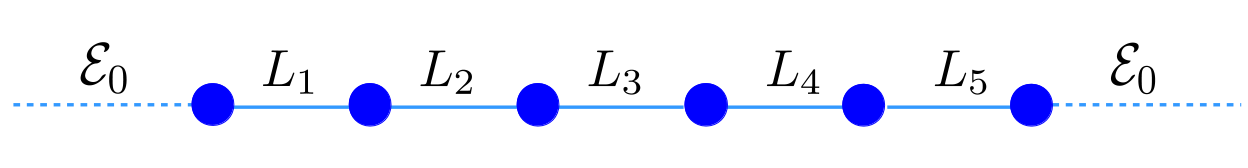
\includegraphics[scale=0.28]{figures/latice4.png}
	\centering
	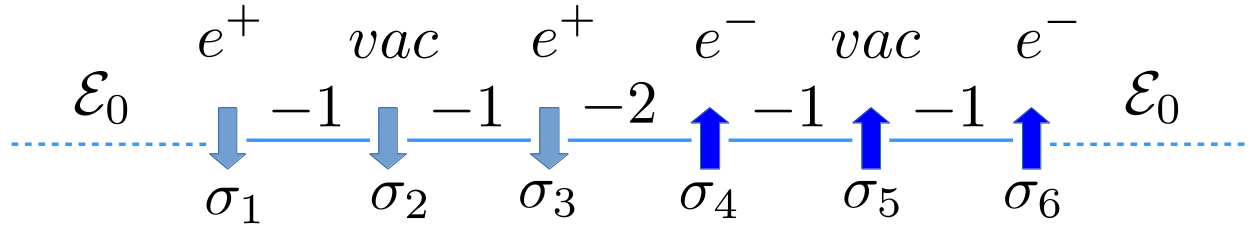
\includegraphics[scale=0.28]{figures/latice5.png}
	\caption{Lattice of $N=6$ spins with the values of electric field $L_n$ fixed by Gauss's law.} \label{fig:l5}
\end{figure}

What is seen in figure \ref{fig:l5} can be summarized as follows, on odd lattice sites

\begin{equation*}
	\uparrow =\ket{0}= \text{vacuum}\Rightarrow L_n = L_{n-1};\quad \downarrow = \ket{1} = \psi_+ = e^+\Rightarrow L_n = L_{n-1} -1,
\end{equation*}

while on even lattice sites

\begin{equation*}
	\uparrow = \ket{1} = \psi_- = e^-\Rightarrow L_n = L_{n-1}+1;\quad \downarrow = \ket{0} = \text{vacuum}\Rightarrow L_n = L_{n-1}.
\end{equation*}

Furthermore, by using relation \eqref{eq:gaussSpin} we can write the electric field Hamiltonian as

\begin{equation}
\xi\sum_n L_n^2 = \xi\sum_n \qty(\mathcal{E}_0 + \frac{1}{2}\sum_{l=1}^{n}\qty[\sigma^z_l + (-1)^l])^2.
\end{equation}

Finally, in order to completely eliminate the operators $U(n;n+1)$, we can make the following gauge transformation

\begin{equation}
\sigma^-_n = \qty[\prod_{l<n}e^{-i\alpha_n}]\sigma^-_n;\quad \sigma^+_n = \qty[\prod_{l<n}e^{i\alpha_n}]\sigma^+_n.
\end{equation}

Plugging transformed operators into the energy term to the electric field we obtain a Hamiltonian written completely in terms the spin content in the sites of the lattice, viz 

\begin{multline}
	H = J\sum_n\qty[\sigma^+_n \sigma^-_{n+1} + \text{h.c}] + \frac{m}{2}\sum_n (-1)^n\sigma^z_n \\
	+ \xi \sum_n \qty(\mathcal{E}_0 + \frac{1}{2}\sum_{l=1}^{n}\qty[\sigma^z_l + (-1)^l])^2.\label{eq:spinHam1}
\end{multline}

In this formulation where the gauge field has been integrated out using Gauss's law. The dynamics of the gauge field is replaced by non-local long-range spin-spin interactions that are an effective description of Coulomb's law in one spatial dimension \cite{Hamer1997}

\section{Effective mass and Coulomb interaction}\label{sec:Coulomb}

Let us now explicitly compute the third term in the Hamiltonian\footnote{Hereafter we are assuming open boundary conditions, but a straightforward modification of the final results yields an expression either for periodic or antiperiodic boundary conditions} \eqref{eq:spinHam1}. Expanding the square we get 

\begin{equation}
\xi \sum_{n=1}^{N-1} \qty(\mathcal{E}_0^2 + \frac{1}{4}\qty(\sum_{l=1}^{n}\qty[\sigma^z_l + (-1)^l])^2 + \mathcal{E}_0\sum_{l=1}^{n}\sigma^z_l),
\end{equation}

the first term is a simple constant energy term we will ignore hereafter, as it is an energy offset that does not affect the physics of the system. The remaining two terms are

\begin{equation}
\xi \sum_{n=1}^{N-1}\frac{1}{4}\qty(\sum_{l=1}^{n}\qty[\sigma^z_l + (-1)^l])^2 + \frac{m_{\mathcal{E}_0}}{2} \sum_{n=1}^{N-1}\sum_{l=1}^{n}\sigma^z_l\label{eq:spinInt},
\end{equation}

with $m_{\mathcal{E}_0} = aq_e^2\mathcal{E}_0$. Moreover, let us note that in the second term in \eqref{eq:spinInt} we can interchange both summations maintaining the condition $l\leq n$, viz

\begin{equation}
m_{\mathcal{E}_0} \sum_{l=1}^{N-1}\sigma^z_l\underbrace{\sum_{n=l}^{N-1}}_{(N-l)}.
\end{equation}

Thus, the background field in \eqref{eq:spinInt} yields a position-dependent effective mass term for the spins in the chain, viz

\begin{equation*}
	\frac{m_{\mathcal{E}_0}}{2} \sum_{n=1}^{N-1}(N-n)\sigma^z_n.
\end{equation*}

The strength of this effective mass term in each site due to the background field is shown in figure \ref{fig:effMassE}

\begin{figure}[htb]
	\centering
	\begin{minipage}{.5\textwidth}
		\centering
		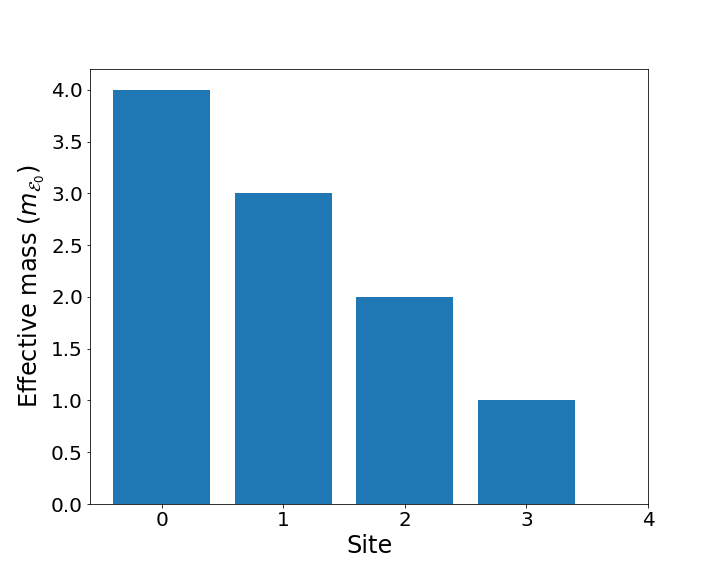
\includegraphics[scale=0.27]{figures/effectiveMass_E_N=5.png}
	\end{minipage}%
	\begin{minipage}{0.5\textwidth}
		\centering
		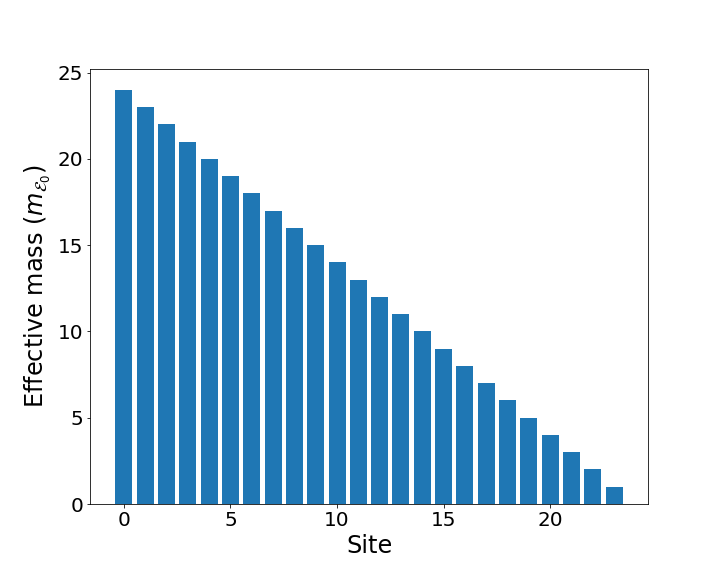
\includegraphics[scale=0.27]{figures/effectiveMass_E_N=25.png}
	\end{minipage}
	\caption{Plot of effective mass term due to the background field $\mathcal{E}_0$ for $N=5$ and $N=25$.}
	\label{fig:effMassE}
\end{figure}


Now, let us simplify the first term in \eqref{eq:spinInt}, to do so we use the equality 

\begin{align}
	&\xi \sum_{n=1}^{N-1}\frac{1}{4}\qty(\sum_{l=1}^{n}\qty[\sigma^z_l + (-1)^l])^2\nonumber\\ 
	&= \frac{\xi}{4} \sum_{n=1}^{N-1}\qty(\sum_{l=1}^{n}\sum_{k=1}^{n}\sigma^z_l\sigma^z_k + 2\underbrace{\sum_{l=1}^{n}(-1)^l}_{-n\mod2}\sum_{k=1}^{n}\sigma^z_{k} + \sum_{l,k=1}^{n}(-1)^{l+k})\label{eq:spinSpinInt},
\end{align}

coming from the standard form of the square of a summation. Note that the last term in \eqref{eq:spinSpinInt} is a constant we can ignore. We have then the following

\begin{equation}
-\frac{m_{\xi}}{2} \sum_{n=1}^{N-1}(n\mod2)\sum_{k=1}^{n}\sigma^z_{k}
+ \frac{\xi}{4} \sum_{n=1}^{N-1}\sum_{l=1}^{n}\sum_{k=1}^{n}\sigma^z_l\sigma^z_k \label{eq:ssInt2}, 
\end{equation}


with $m_\xi = q_e^2a/2 $. Note that again the first term of \eqref{eq:spinSpinInt} is a position dependent effective fermion mass analogous to the one generated by the background field $\mathcal{E}_0$. The strength of the effective mass term,  $m_{\xi}$, in each site is shown in figure \ref{fig:effMassXi}.\\

\begin{figure}[htb]
	\centering
	\begin{minipage}{.5\textwidth}
		\centering
		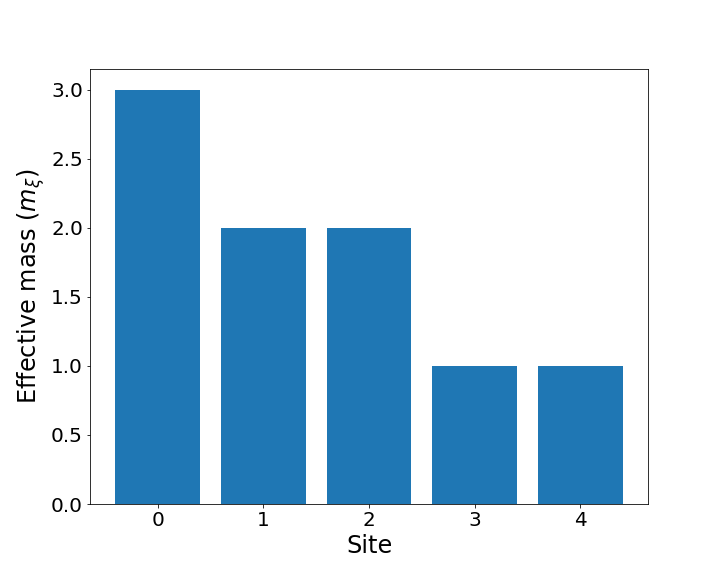
\includegraphics[scale=0.27]{figures/effectiveMass_xi_N=5.png}
	\end{minipage}%
	\begin{minipage}{0.5\textwidth}
		\centering
		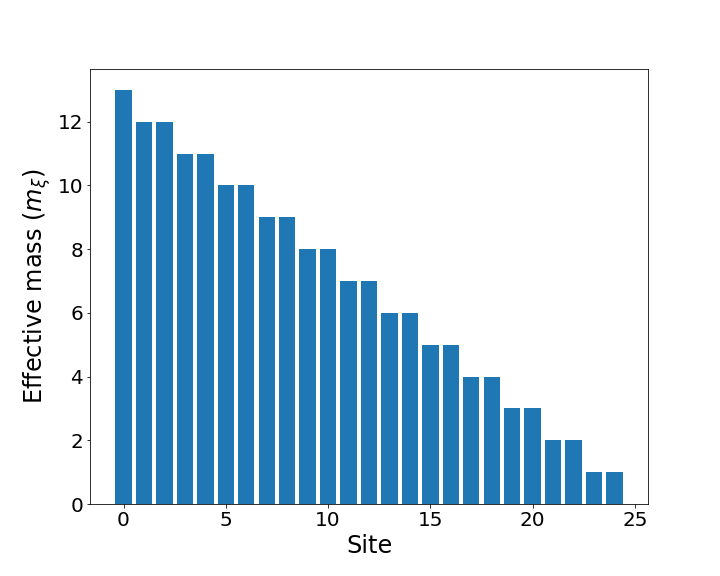
\includegraphics[scale=0.27]{figures/effectiveMass_xi_N=25.png}
	\end{minipage}
	\caption{Plot of effective mass term, $m_\xi$, for $N=5$ and $N=25$.}
	\label{fig:effMassXi}
\end{figure}

Finally, let us focus our attention to the second term in \eqref{eq:ssInt2}. The two inner summations can be simplified by using the fact that $(\sigma^z)^2 = 1$, which yields a constant term we will ignore. And $\comm{\sigma^z_l}{\sigma^z_m}=0$, implying that the crossed terms appear twice, viz

\begin{equation}
\frac{\xi}{4} \sum_{n=1}^{N-1}\sum_{l=1}^{n}\sum_{k=1}^{n}\sigma^z_l\sigma^z_k = \frac{\xi}{2} \sum_{n=1}^{N-1}\sum_{l=1}^{n}\sum_{k<l}\sigma^z_l\sigma^z_k.
\end{equation}



Using the same interchange we used in \eqref{eq:spinInt}, and enforcing the condition $l\leq n$ we obtain that

\begin{equation}
\frac{\xi}{2} \sum_{l=1}^{N-1}\sigma^z_l\underbrace{\sum_{n=l}^{N-1}}_{(N-l)}\sum_{k=1}^{l-1}\sigma^z_k,
\end{equation}

interchanging the two summations one last time keeping in mind that $k<l$, we obtain the final expression for this term

\begin{equation}
J_{zz} \sum_{n=1}^{N-2}\sum_{m=n+1}^{N-1}(N-m)\sigma^z_n\sigma^z_m = J_{zz} \sum_{n<m}C_{nm}\sigma^z_n\sigma^z_m
\end{equation}

with $J_{zz} = q_e^2a/2$. We can plot the strength of the Coulomb $C_{nm}$ interaction in the lattice, this is shown in figure \ref{fig:coul}. This term is, as previously stated, long-range spin-spin interactions that are an effective description of Coulomb's law in our system.

\begin{figure}[htb]
	\centering
	\begin{minipage}{0.5\textwidth}
		\centering
		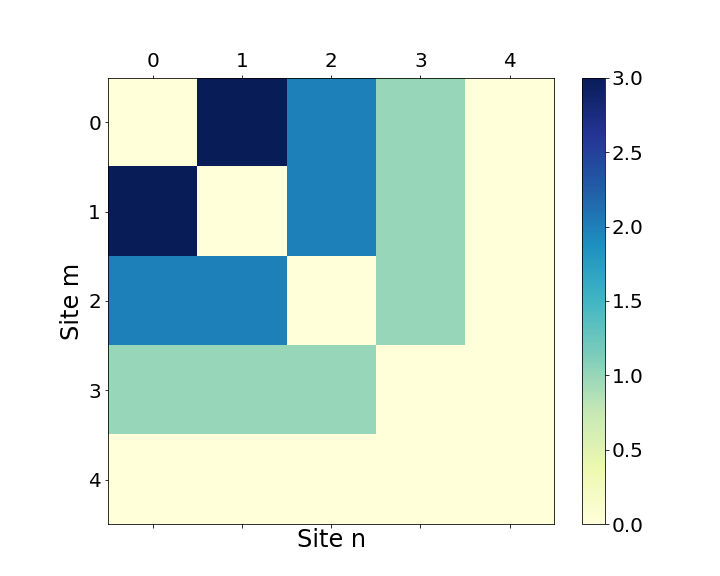
\includegraphics[scale=0.27]{figures/c_ij_N=5.png}
	\end{minipage}%
	\begin{minipage}{0.5\textwidth}
		\centering
		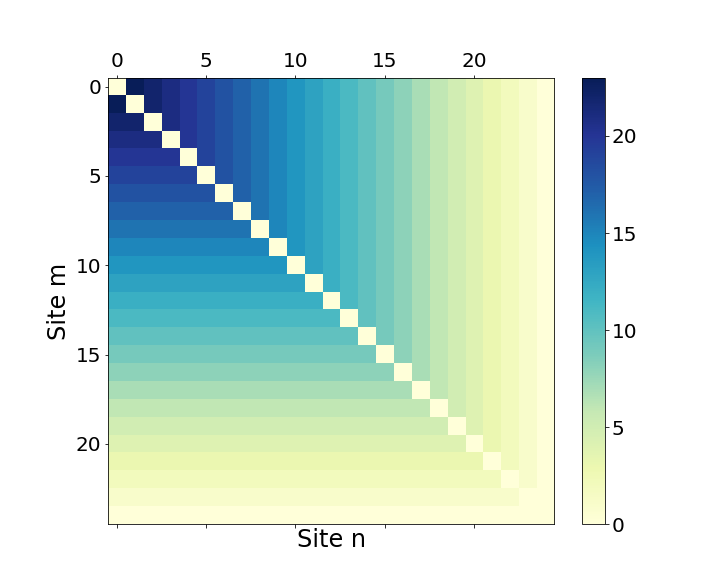
\includegraphics[scale=0.27]{figures/c_ij_N=25.png}
	\end{minipage}
	\caption{Plot of Coulomb strength interaction $C_{nm}$ between spins in the lattice for $N=5$ and $N=25$.}
	\label{fig:coul}
\end{figure}

After this calculation the Hamiltonian, which is expressed solely in terms of spin variables is
\begin{equation}
H = H_{p-a} + H_{\text{mass}} + H_{\text{eff. mass}} + H_{\text{Coulomb}}
\end{equation}

such that
\begin{equation*}
	H_{p-a}  = J \sum_{n=1}^{N-1}[\sigma^+_n \sigma^-_{n+1}  + \sigma^+_{n+1}\sigma^-_{n}  ]
\end{equation*}

is a particle-antiparticle creation term.

\begin{equation*}
	H_{mass}  = \frac{m}{2}\sum_n (-1)^n\sigma^z_n
\end{equation*}

is the fermion mass term.

\begin{align*}
	H_{\text{eff. mass}} &=  \frac{m_{\mathcal{E}_0}}{2} \sum_{n=1}^{N-1}(N-n)\sigma^z_n  - \frac{m_\xi}{2} \sum_{n=1}^{N-1}\sum_{k=1}^{n}(n\mod2)\sigma^z_{k}\\
	&= \frac{m_{\mathcal{E}_0}}{2}\sum_{n=1}^{N-1}C_n\sigma^z_n - \frac{m_\xi}{2} \sum_{n=1}^{N-1} D_n \sigma^z_n
\end{align*}

is the effective fermion masses term. And

\begin{equation*}
	H_{\text{Coulomb}} = J_{zz} \sum_{n<m}C_{nm}\sigma^z_n\sigma^z_m
\end{equation*}

is the Coulomb interaction between the spin in the lattice. It is very important to note that as a consequence of the  restriction imposed by Gauss's law the physical Hilbert space of our lattice theory is the space of eigenstates of $\sigma^z$ in each lattice site (with size $2^N$), viz

\begin{equation}
\mathscr{H} =\bigotimes_{i=1}^N\ket{s_i}
\end{equation}

\section{Comment and conclusion}

Throughout this chapter, we have explored the formulation and physics of the lattice Schwinger model. First in section \ref{sec:latticeFormulation}, we described how a discretization of the continuum model could be made using Kogut-Susskind fermions. These fermions decompose the two-component two-dimensional spinor into a single component canonical fermion field in a staggered lattice, where the particles reside in the even lattice sites while the antiparticles are in the odd lattice sites. This decomposition avoids the \emph{fermion doubling problem}, that is the appearance of various non-physical fermionic excitations as a consequence of a naive discretization of a continuum fermionic model \cite{Susskind1977}. With this in mind and having as a reference the analytic solution of the XY-model (cf. \ref{sec:XYmodel}) we introduced a Jordan-Wigner transformation and showed the equivalence of the free lattice Schwinger model with an XX spin chain. The equivalence to the XX-model without a transverse magnetic field in the case of $m=0$, and with an XX-chain with a staggered transverse magnetic field in the case $m>0$.\\

Subsequently, in subsection \ref{ssec:operators}, we introduced the electric field into the lattice having as a guiding principle the method of gauge invariant point splitting to render the Lattice Hamiltonian gauge invariant. We showed that the lattice version of the electric field is realized by a quantum rotor residing in the links between the fermions (or spins). Having this result about the electric field it was easy to incorporate the background field into the formulation, as it boils down to adding the background field $\mathcal{E}_0$ to the electromagnetic Hamiltonian. We commented on how the discrete lattice model inherits the critical behavior of the continuum model. This behavior can be explored by studying the order parameters of axial fermion density $\Lambda$ and of density of chiral condensate $\Gamma$.\\

Moreover, we showed the by imposing Gauss's law we can restrict the Hilbert space to the subspace of physical states and integrate out the gauge field degrees of freedom altogether from the lattice system. Hence, the Hamiltonian of the system is finally written solely in terms of the spin (or fermion content) of the lattice, namely

\begin{multline*}
	H = J\sum_n\qty[\sigma^+_n \sigma^-_{n+1} + \text{h.c}] + \frac{m}{2}\sum_n (-1)^n\sigma^z_n \\
	+ \xi \sum_n \qty(\mathcal{E}_0 + \frac{1}{2}\sum_{l=1}^{n}\qty[\sigma^z_l + (-1)^l])^2.
\end{multline*}

Finally, in section \ref{sec:Coulomb}, we showed that the electromagnetic term in the Hamiltonian of the lattice model, after imposing Gauss's law, gives rise to three non-trivial interaction terms in the system. First, it gives rise to an effective mass term which depends on the position of the spin within the chain. Secondly, it generates another effective mass term appears due to the presence Background field $\mathcal{E}_0$. Both this contributions generate the following net effective mass Hamiltonian


\begin{equation*}
	H_{\text{eff. mass}} = \frac{m_{\mathcal{E}_0}}{2}\sum_{n=1}^{N-1}C_n\sigma^z_n - \frac{m_\xi}{2} \sum_{n=1}^{N-1} D_n \sigma^z_n.
\end{equation*}

The magnitude of the effective mass $C_n$ and $D_n$ are plotted in figures \ref{fig:effMassE} and \ref{fig:effMassXi} respectively. Lastly, another term arising from the electromagnetic Hamiltonian is a spin-spin interaction which is linear in distance, being an effective description of Coulomb's interaction in the system. This term is described by the Hamiltonian

\begin{equation*}
	H_{\text{Coulomb}} = J_{zz} \sum_{n<m}C_{nm}\sigma^z_n\sigma^z_m, 
\end{equation*}

where the strength of the coupling $C_{nm}$ is plotted in figure \ref{fig:coul}. This term of spin-spin interaction breaks the integrability of the lattice system and forces us to abandon the hope of solving the system analytically. Rather, we must appeal to numerical simulation in order to study the dynamics and physically relevant quantities of the system. This endeavor will be presented in the next chapter.